\section{W12 - Lean Synchronization}
\subsection{History of Lean }
\subsubsection{Lean Management and Just in Time (JIT)}
For Slack et al., the following terms are synonymous
\begin{itemize}
	\item continuous flow manufacture
	\item high value-added manufacture
	\item stockless production
	\item low-inventory production
	\item fast-throughput manufacturing
	\item lean manufacturing
	\item Toyota production system
	\item short cycle-time manufacturing
\end{itemize}
\subsubsection{Toyota Simultaneously Increases Quality and Productivity}
\subsubsection{Introductory Movie on Lean }
\subsubsection{JIT Definitions}
\subsubsection{Lean Optimizes 3 Aspects Simultaneously}
\subsubsection{Successful lean projects are based on 3 preconditions}
\subsection{3 Value Destroyers}
\subsubsection{The 3 Value Destroyers: Waste, Variability, and Inflexibility }
\subsubsection{The 7+1 Types of Waste (= muda\index{muda})}
\begin{enumerate}
\item overproduction
\item waiting time
\item transport
\item over-process/poor process
\item inventory
\item motion
\item defective gooods
\item \textit{people's unused potential}
\end{enumerate}
\subsubsection{There Is a Gray Area Between Waste and Value-Added Activity}
\subsubsection{Variability: 5 Typical Reasons}
\begin{itemize}
\item Enviroment
\item People
\item Process/Tools
\item Material
\item Information
\end{itemize}
\subsubsection{Inflexibility: We Are Used to Waste}
\subsection{The Lean Toolbox}
\subsubsection{How to Become Lean – Example of a Toolset}
\begin{enumerate}
	\item Analyze processes
	\item Reduce inventories 
	\item Optimize process technology
	\item Standardize
	\item Change over quickly (SMED)
	\item Implement flow/ level	scheduling (Heijunka\index{Heijunka})
\end{enumerate}
\subsubsection{ There Are 3 Types of Processes}
\begin{enumerate}
	\item What the process really is
	\item What we think the process is
	\item What the process should be
\end{enumerate}
\subsubsection{Airbus A340-300 Maintenance Services}
\subsubsection{Spaghetti Diagrams}
\subsubsection{Reducing Waste}
\subsubsection{Spaghetti Diagram in a Hospital:	Preparing the Surgical Carts for the OR}
\subsubsection{ The Problem with Inventory}
\subsubsection{ Process Technology (Small-Scale Technology)}
\subsubsection{ Example of Standardized Work}
\subsubsection{Definition of Standardized Work\index{Standardized!Work}}
Standardized work is the currently best way to safely complete an activity with the proper outcome and the highest quality
\subsubsection{How Pit Stop Teams Manage Their Fast	Tire Changes?}
\subsubsection{Reducing Set-Up Reduces Inventory: SMED – Single Minute Exchange of Die}
D=demand\\
$C_O$ = ordering (set-up) cost = \textsterling
400 / order\\
$C_h$ = holding cost = \textsterling
900 / item / yr = \textsterling
900\\
Eonomic order quantity (EOQ\index{EOQ}):\\
$\sqrt{\frac{2 \cdot D \cdot C_O}{C_h}}$ = $\sqrt{\frac{2 \cdot 5000 \cdot 400}{900}}$ = 67 \\
Reducing the order (set-up) cost from \textsterling
400 to \textsterling
100:\\
$\sqrt{\frac{2 \cdot 5000 \cdot 100}{900}}$ = 33.33\\
\textbf{SMED}\\
Single minute exchange of die ist eine Messgr\"osse wie lange man zur Umr\"ustung einer Maschine braucht vom letzten produzieren Teil bis zum ersten neuen
\subsubsection{Levelled Scheduling (Heijunka\index{Heijunka}) Balances the Mix of Products Produced every Day}
Der Mix und das Volumen zwischen versch. Stationen soll gleich behalten werden. Das f\"uhrt zu kleinere Menge die verschoben werden m\"ussen, kleinere Lager n\"otig, Fehler werden schneller aufgedeckt, einfachere Planung
\subsubsection{Levelled Scheduling (Heijunka\index{Heijunka}) Balances the Mix of Products Produced every Day (Continued)}
\subsubsection{Delivering Smaller quantities More Frequently Can Reduce Inventory Levels}
\subsubsection{Basics of Material Flow: Credo of Lean Production}
\index{Lean!Production Credo}
Eliminate the \textbf{U}nnecessary -> \textbf{S}implify the necessary -> \textbf{A}utomate Simplified processes = \textbf{''USA\index{USA}''}
\subsubsection{How to Become Lean – Example of a Toolset }\label{sssec:becomelean}
\begin{enumerate}
	\item Analyze processes
	\item Reduce inventories
	\item Optimize process technology
	\item Standardize
	\item Change over quickly (SMED)
	\item Implement flow/ level scheduling (Heijunka)
\end{enumerate}
\subsubsection{Read More on Lean Banking on Moodle…}
\subsubsection{The 3 Step Approach to Lean Banking}
\begin{enumerate}
	\item Identify \textbf{customer needs}
	\item Understand \textbf{root causes} for poor performance
\item Create \textbf{behavioral change}
\end{enumerate}
\subsubsection{Poor Performance – Examples of Wastes in a Mortgage Process (Muda\index{Muda})}
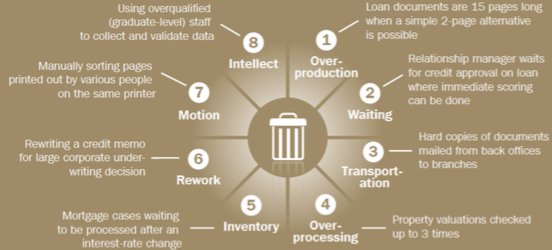
\includegraphics[width=1\textwidth]{W12/poorperformance}
\subsubsection{How to Achieve the Transformation? Use your Operations	Knowledge – Example Capacity}
\subsubsection{Lean Banking Can Transform Every Part of a Bank}
